\section{Android Apps}\label{sec:sota_apps}
In this section we investigate the state of the art for synchronized streaming of music between different mobile devices.
This means that we will look at apps which is capable of synchronizing the playback of music between several mobile devices.
We found three apps capable this:
\begin{itemize}
    \item SoundSeeder
    \item AmpMe
    \item Chorus
\end{itemize}

These apps are found by searching sources like Google\footnote{https://www.google.dk with search term ``android sync music playback''}, YouTube\footnote{https://www.youtube.com/}, App Store\footnote{https://itunes.apple.com/dk}, and Google Play Store\footnote{https://play.google.com/store} and from recommendations on forums. 
A criteria for an app was that the it must not be depreciated or abandoned by its developers.
The way to estimate this was done by looking at the last update date on Google Play Store and App Store.
For instance if an app had not been updated for a long time, e.g. since 2013 and it do not support new devices, it is probably abandoned.

To clarify, Google Play Store and App Store are the official place to install or buy apps for Android and iOS devices respectively.

The three apps all use a master/slave connection.
All three apps use different terms for their setup, for clarification we generalise these terms. 
We call the device which selects the music and streams it, the master.
The devices which connects to the master (SoundSeeder calls it ``Speaker''), are referred to as slaves.

\subsection{SoundSeeder}\label{subsec:soundseeder}
SoundSeeder\footnote{http://soundseeder.com} is an app made by JekApps. 
The used version of the app is 1.6.5.

It is compatible with Android 4.1 and above, for older versions of Android (2.2 -- 4.0),
another app called SoundSeeder Speaker makes it possible for the device to be used as a slave.

SoundSeeder also provides a Java application for compatibility with other platforms e.g. Windows, macOS and Linux.
SoundSeeder does not support iOS and Windows Phone\cite{soundseeder_ios}.

The app consists of a top menu and a burger menu at he left side, as seen on \cref{fig:soundseeder_screenshot}.
In the burger menu, the user can choose the different playback possibilities and switch to slave mode.
The main view of the app is a music player, where the music can be controlled as any other music player. 
To play music to other devices as a master, press the ``add music button'' in the top menu,
choose the source of the music and choose the preferred music, and press play. 

To connect to a playing master device as a slave, select the speaker mode from the burger menu and if it finds the device, it connects automatically.
It took a bit of time before the slave device found the master device, which can seem confusing and make users think they need to connect manually with an IP address. 

The process of joining, when the slave is given the time, is rather simple.
In regard to the user interface, it is clotted with features and menus, which makes the app hard to navigate.
The design of the app is old and not pretty.

SoundSeeder streams music via Wi-Fi, 
which means that all phones have to be on the same network\cite{soundseether_faq}, it is also possible to use an ad--hoc network (Android Hotspot).
In regard to the master's music source, it can be Google Music, online radio stations, UPnP and DLNA devices, local media, and YouTube if using semperVidLinks\footnote{\url{https://play.google.com/store/apps/details?id=com.semperpax.sempervidlinksFree}}, an app for extracting video links.
SoundSeeder also supports streams from external sources, e.g. a microphone or AUX device. 
The supported media formats depend on the used master device and its Android version.\cite{soundseether_faq}

SoundSeeder synchronizes the audio playback when a slave connects, but it can also be done manually on the slave device. 
On \cref{fig:soundseeder_slider}, the manual synchronization adjustment for SoundSeeder can be seen.
This slider is used in the case that the music is not fully synchronized, the slider goes from $-400 ms$ up to $+400 ms$, in steps of $10 ms$.
Furthermore there is also an auto synchronization button in the top menu and on the slider menu window. 

SoundSeeder is free to install but the free version only allows two slave devices to connect for up to 15 minutes at a time.
The full app costs 39.90 DKK. 

\begin{figure}[h!]
    \setlength{\fboxsep}{0pt}
    \setlength{\fboxrule}{2pt}
    \begin{minipage}[b]{0.45\textwidth}
        \centering    
        \fbox{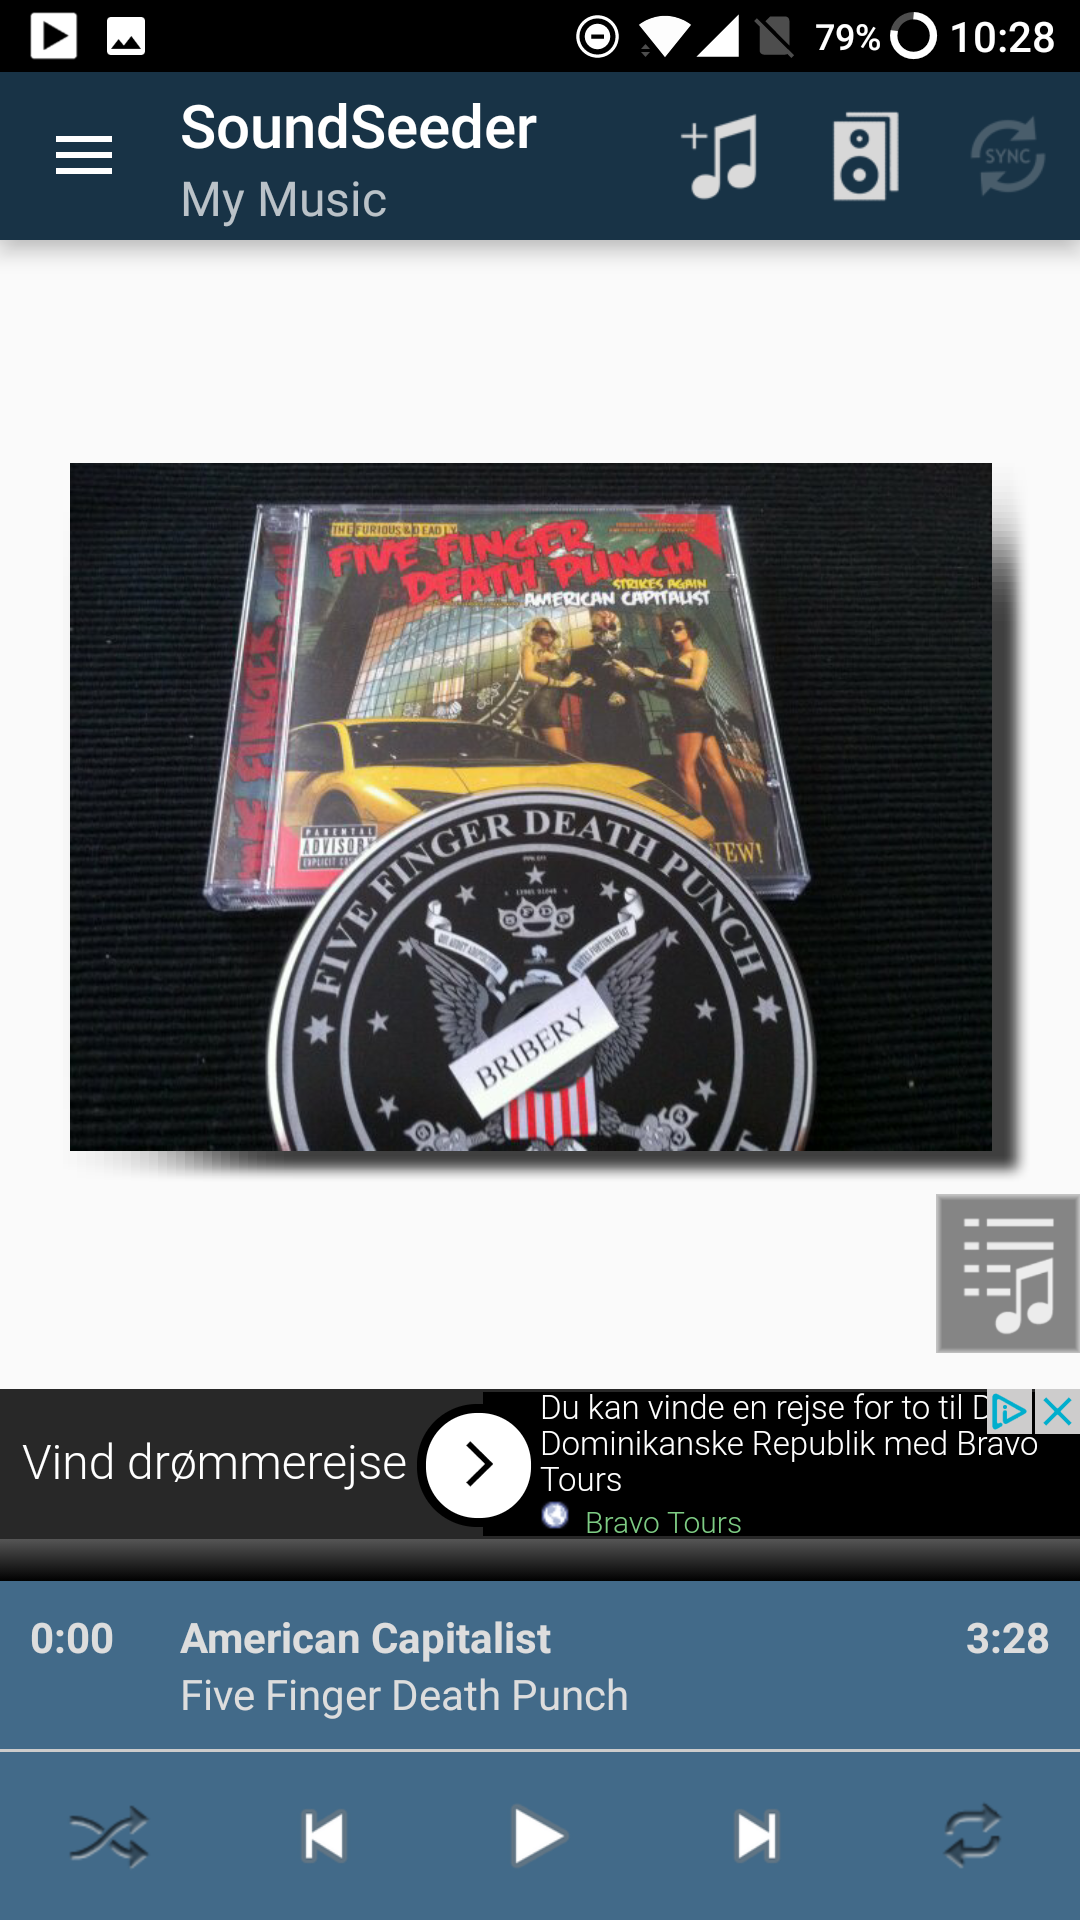
\includegraphics[width=0.65\textwidth]{img/sota/soundseeder.png}}
        \caption{A screenshot of SoundSeeder when the app is opened.}\label{fig:soundseeder_screenshot}
    \end{minipage}
    \hfill
    \begin{minipage}[b]{0.45\textwidth}
        \centering
        \fbox{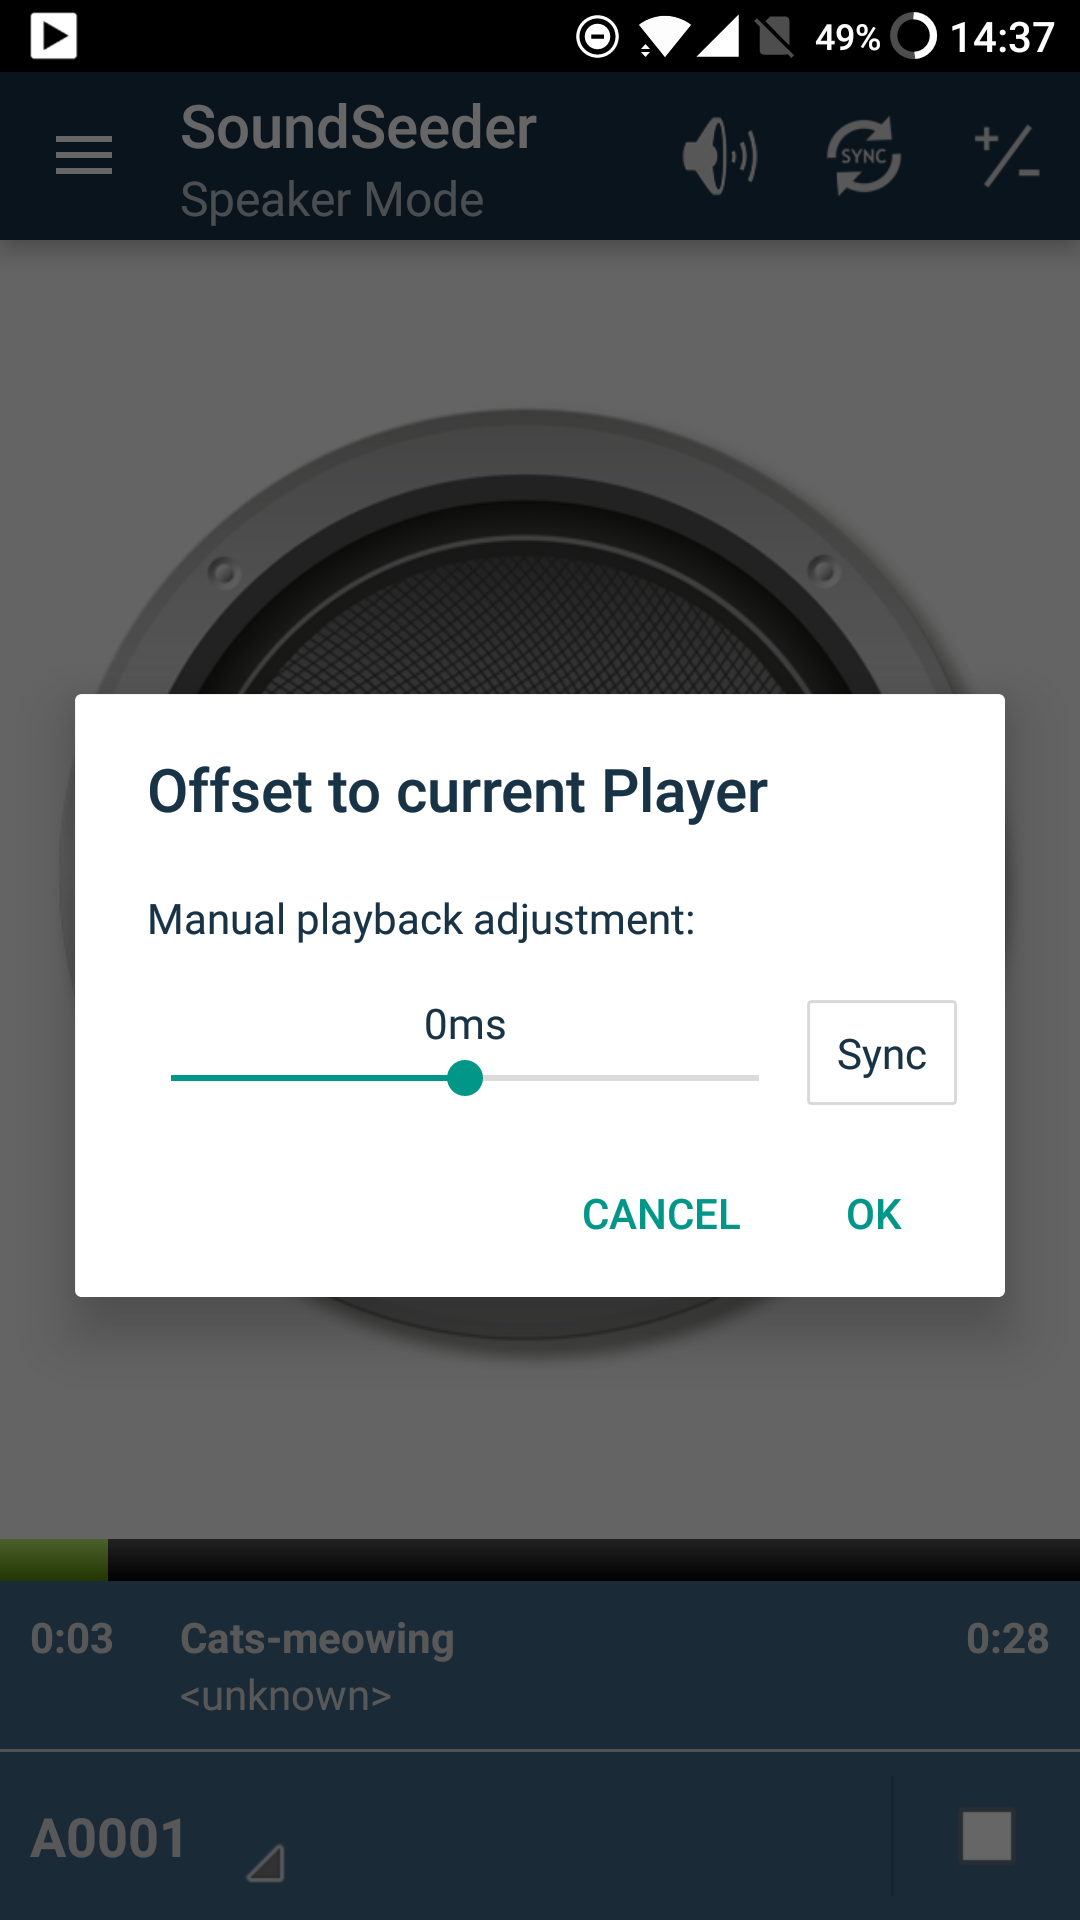
\includegraphics[width=0.65\textwidth]{img/sota/soundseeder_slider.png}}
        \caption{A screenshot of SoundSeeder's synchronization slider.}\label{fig:soundseeder_slider}
    \end{minipage}
\end{figure}

\subsection{AmpMe}\label{subsec:ampme}
The second app is AmpMe\footnote{\url{http://www.ampme.com}}, made by Amp Me Inc.
The used version of the app is 5.1.1.
It supports Android 4.1 or newer and iOS 9.0 or newer.

In AmpMe the group of devices is called ``a party''.
When AmpMe is opened, it either displays the nearby parties or encourage you to create your own. 
If a party if found, you can join it as a slave and play the master's music.
If no party is found, or you want to create your own, you can choose to start it by choosing between Spotify, 
YouTube, your own music library, or SoundCloud as music source, as shown on \cref{fig:ampme_screenshot}. 
When a source and music is chosen, a player appears with the music playing,
and your device works as a master.

It is very intuitive to join a party, or host one yourself and play music.
Furthermore the interface is modern, minimalistic, and pleasant to use and look at. 

In order to stream music from a master to slaves, AmpMe requires internet, in the form of WiFi or mobile data.
This means that the connected devices can be on WiFi, mobile data or another network, as long there is Internet access. 

In AmpMe, the music is automatically synchronized upon party creation,
but if there is a delay, it can be synchronized manually on the slave.
On \cref{fig:ampme_screenshot} the slider to manually synchronize can be seen.
The slider goes from an offset of $-15$ to $+15$ arbitrary offset units.

AmpMe is free to use in both Google Play and App Store.\cite{amp_faq}\cite{amp_play}\cite{amp_itunes}

\begin{figure}[h!]
\setlength{\fboxsep}{0pt}
    \setlength{\fboxrule}{2pt}
    \begin{minipage}[b]{0.45\textwidth}
        \centering
        \fbox{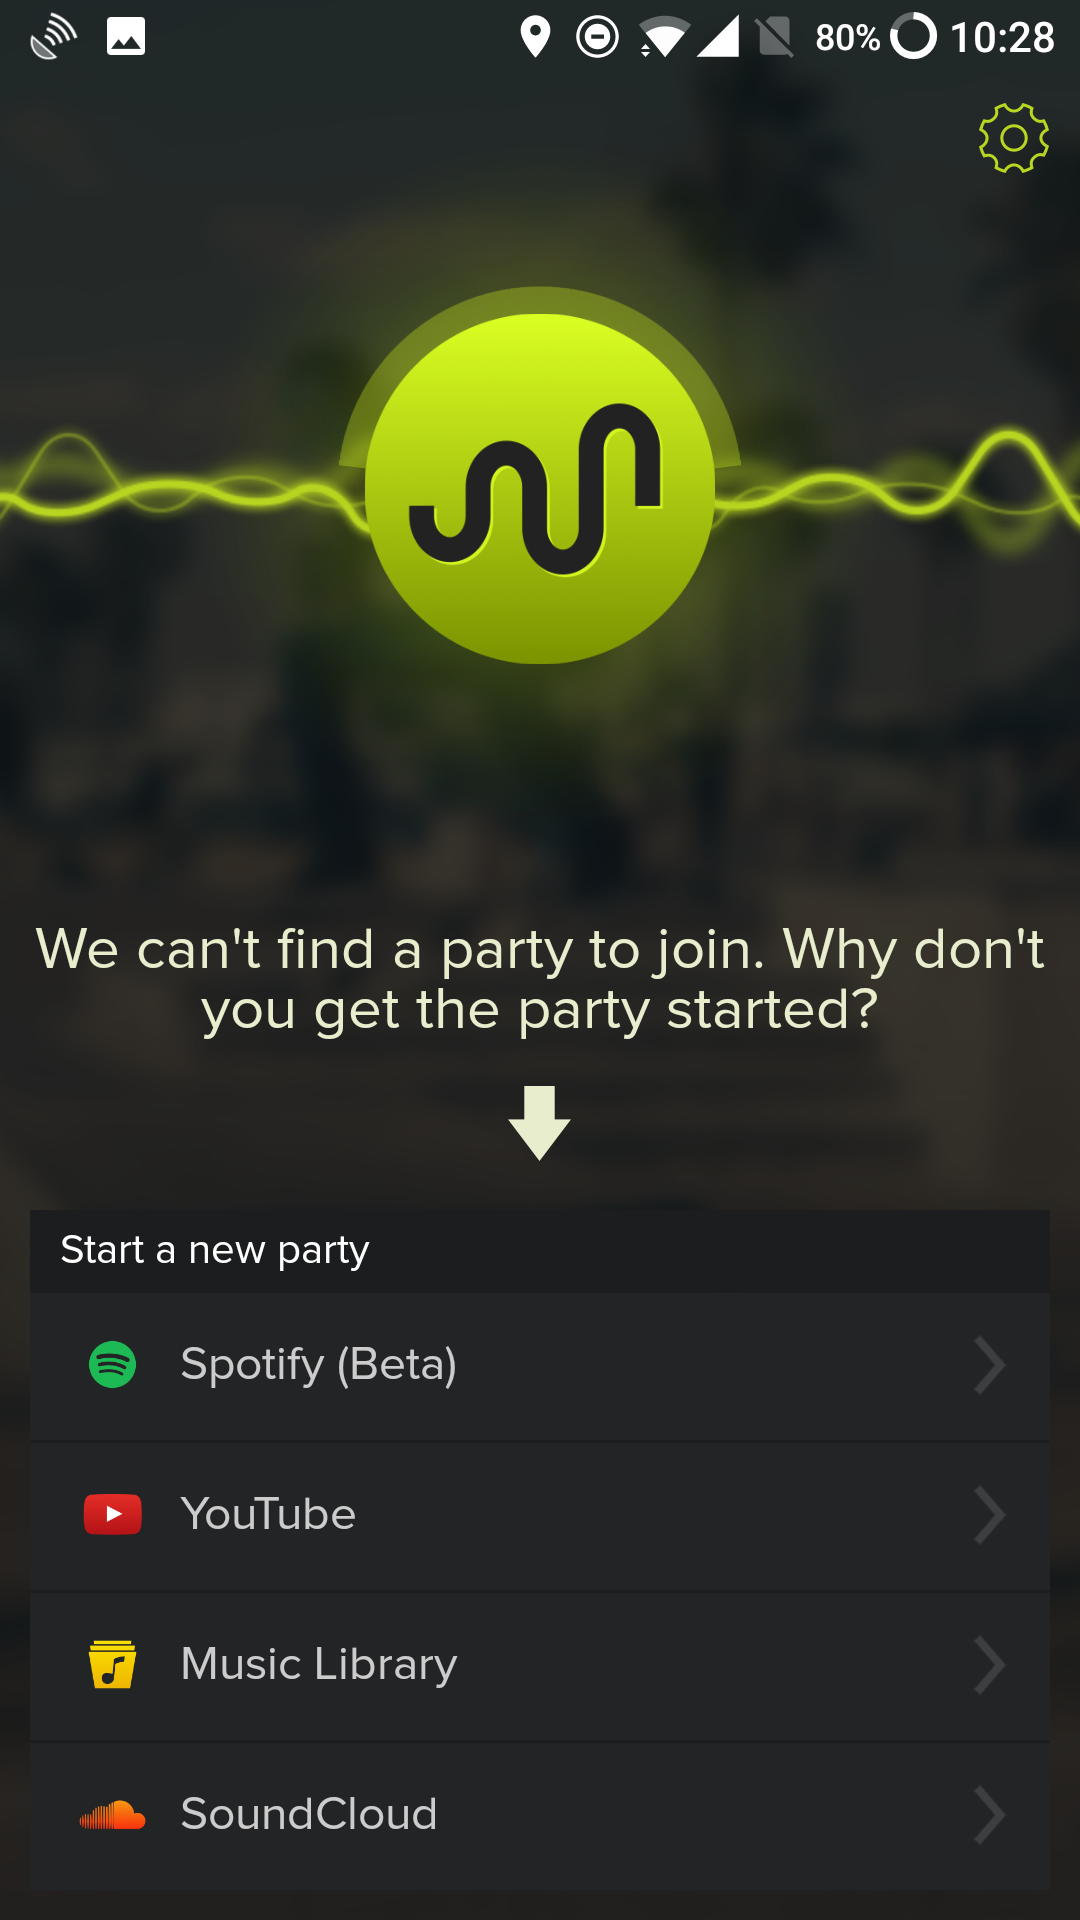
\includegraphics[width=0.65\textwidth]{img/sota/ampme.png}}
        \caption{A screenshot of AmpMe when the app is opened.}\label{fig:ampme_screenshot}
    \end{minipage}
    \hfill
    \begin{minipage}[b]{0.45\textwidth}
        \centering
        \fbox{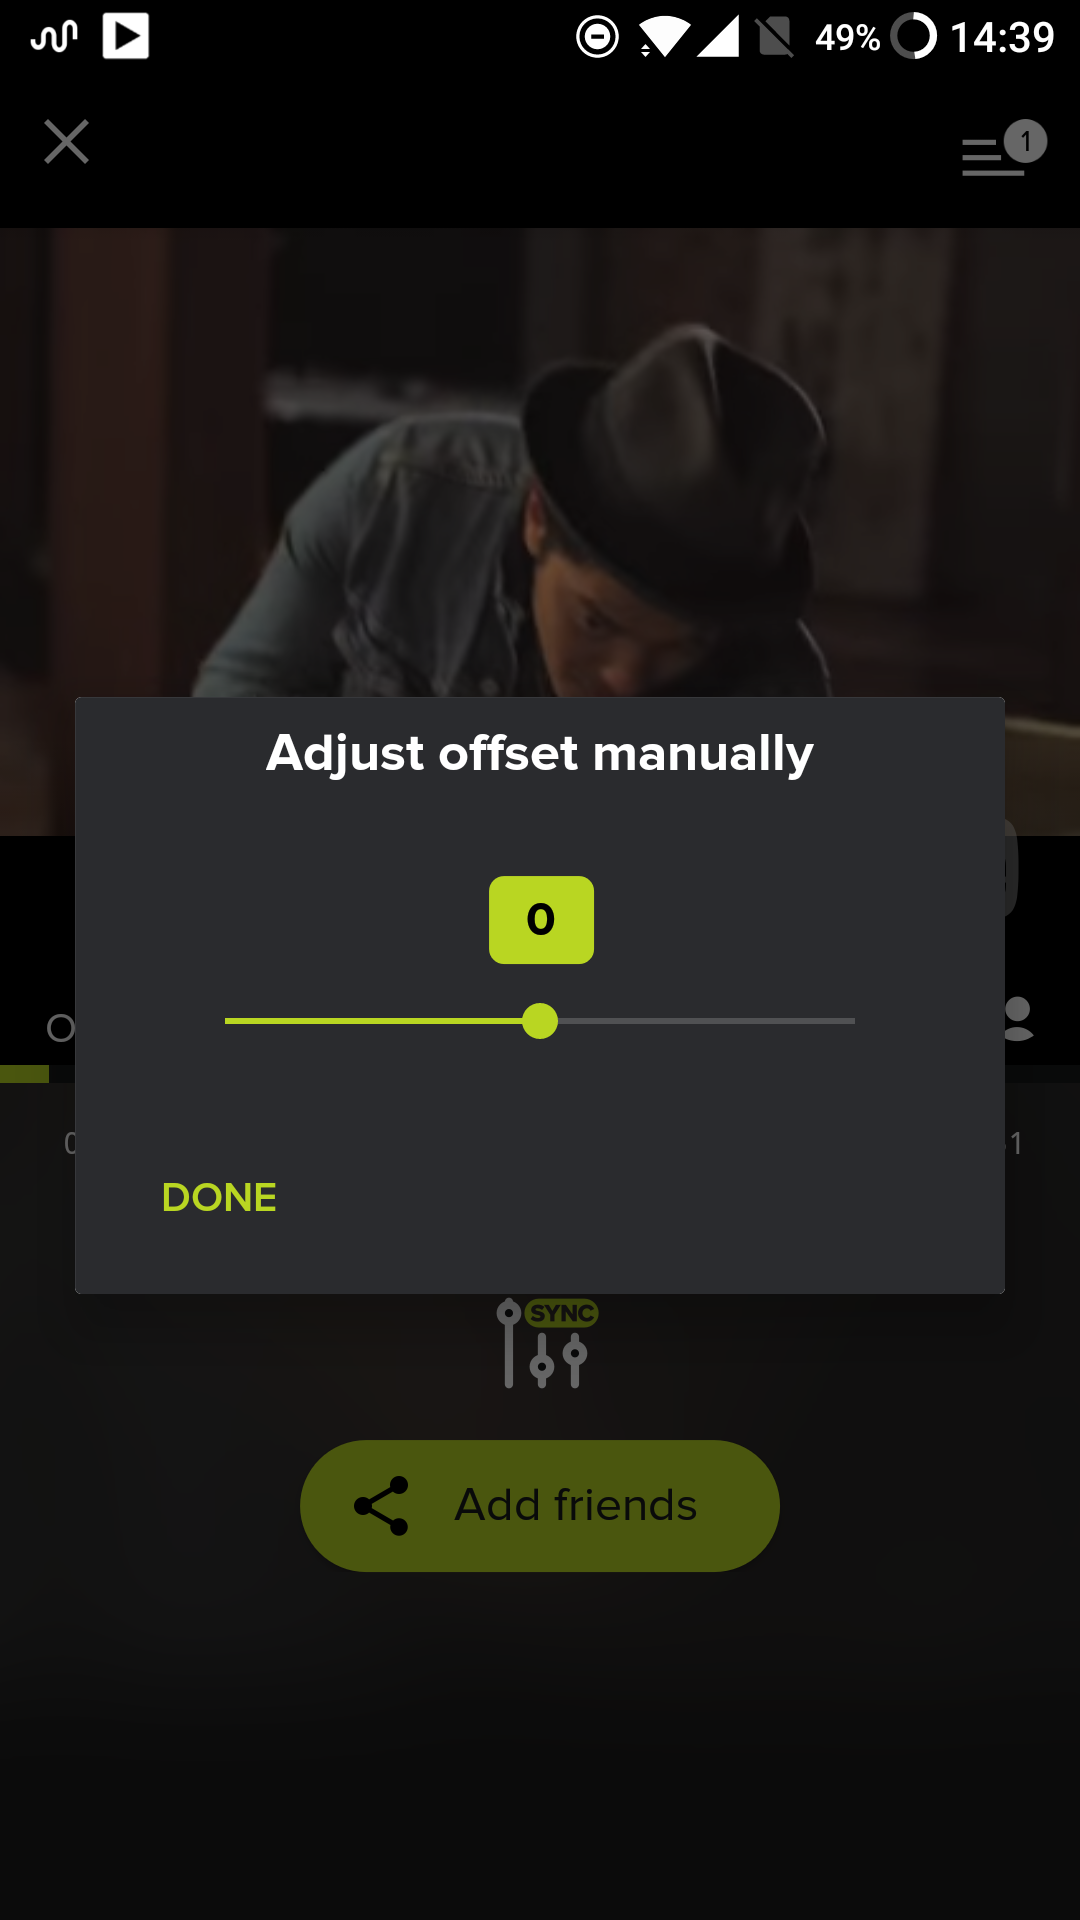
\includegraphics[width=0.65\textwidth]{img/sota/ampme_slider.png}}
        \caption{A screenshot of AmpMe's synchronization slider.}\label{fig:ampme_slider}
    \end{minipage}
\end{figure}

\subsection{Chorus}\label{subsec:chorus}
The final app is called Chorus\footnote{\url{https://play.google.com/store/apps/details?id=com.avrapps.chorus}} and is made by AVR APPS.
The used version of the app is 2.1.
It supports Android 4.0 or newer, AVR APPS mention an iOS app, but the App Store page returns that the app is not available in our region,
when opened in iTunes\footnote{\url{https://itunes.apple.com/app/chorus/id894014439}}.

To share music between devices, WiFi or mobile hotspot is required,
which means that all devices have to be on the same network.
Chorus only supports playback of local media, so the music have to be in memory on the master device.

When the app is opened, it looks like a regular music player, as seen on \cref{fig:chorus_screenshot}.
Music is added by pressing the small plus sign in the right bottom corner. 
When that music is added, Chorus streams the music to connected slave devices.
To connect to a master device playing music, you press the menu button in the right top corner, and press join.
Here a menu pops up with devices playing on the network, and if you select the device shown, it connects as a slave and starts playing.
We encountered a scenario where the app just kept loading when attempting to join an active network, after a restart of the app it worked.

It is intuitive to use the app, it is very minimalistic hence easy to navigate.
The design is a bit old but its simplicity makes up for it.

Chorus supports manual and automatic synchronization.
On \cref{fig:chorus_screenshot} the synchronization slider can be seen,
it slides from $-400ms$ to $+400ms$, in steps of $10 ms$.

The app is free to download and use without any adds.\cite{chrous_play} 

\begin{figure}[h!]
    \setlength{\fboxsep}{0pt}
    \setlength{\fboxrule}{2pt}
    \begin{minipage}[b]{0.45\textwidth}
        \centering
        \fbox{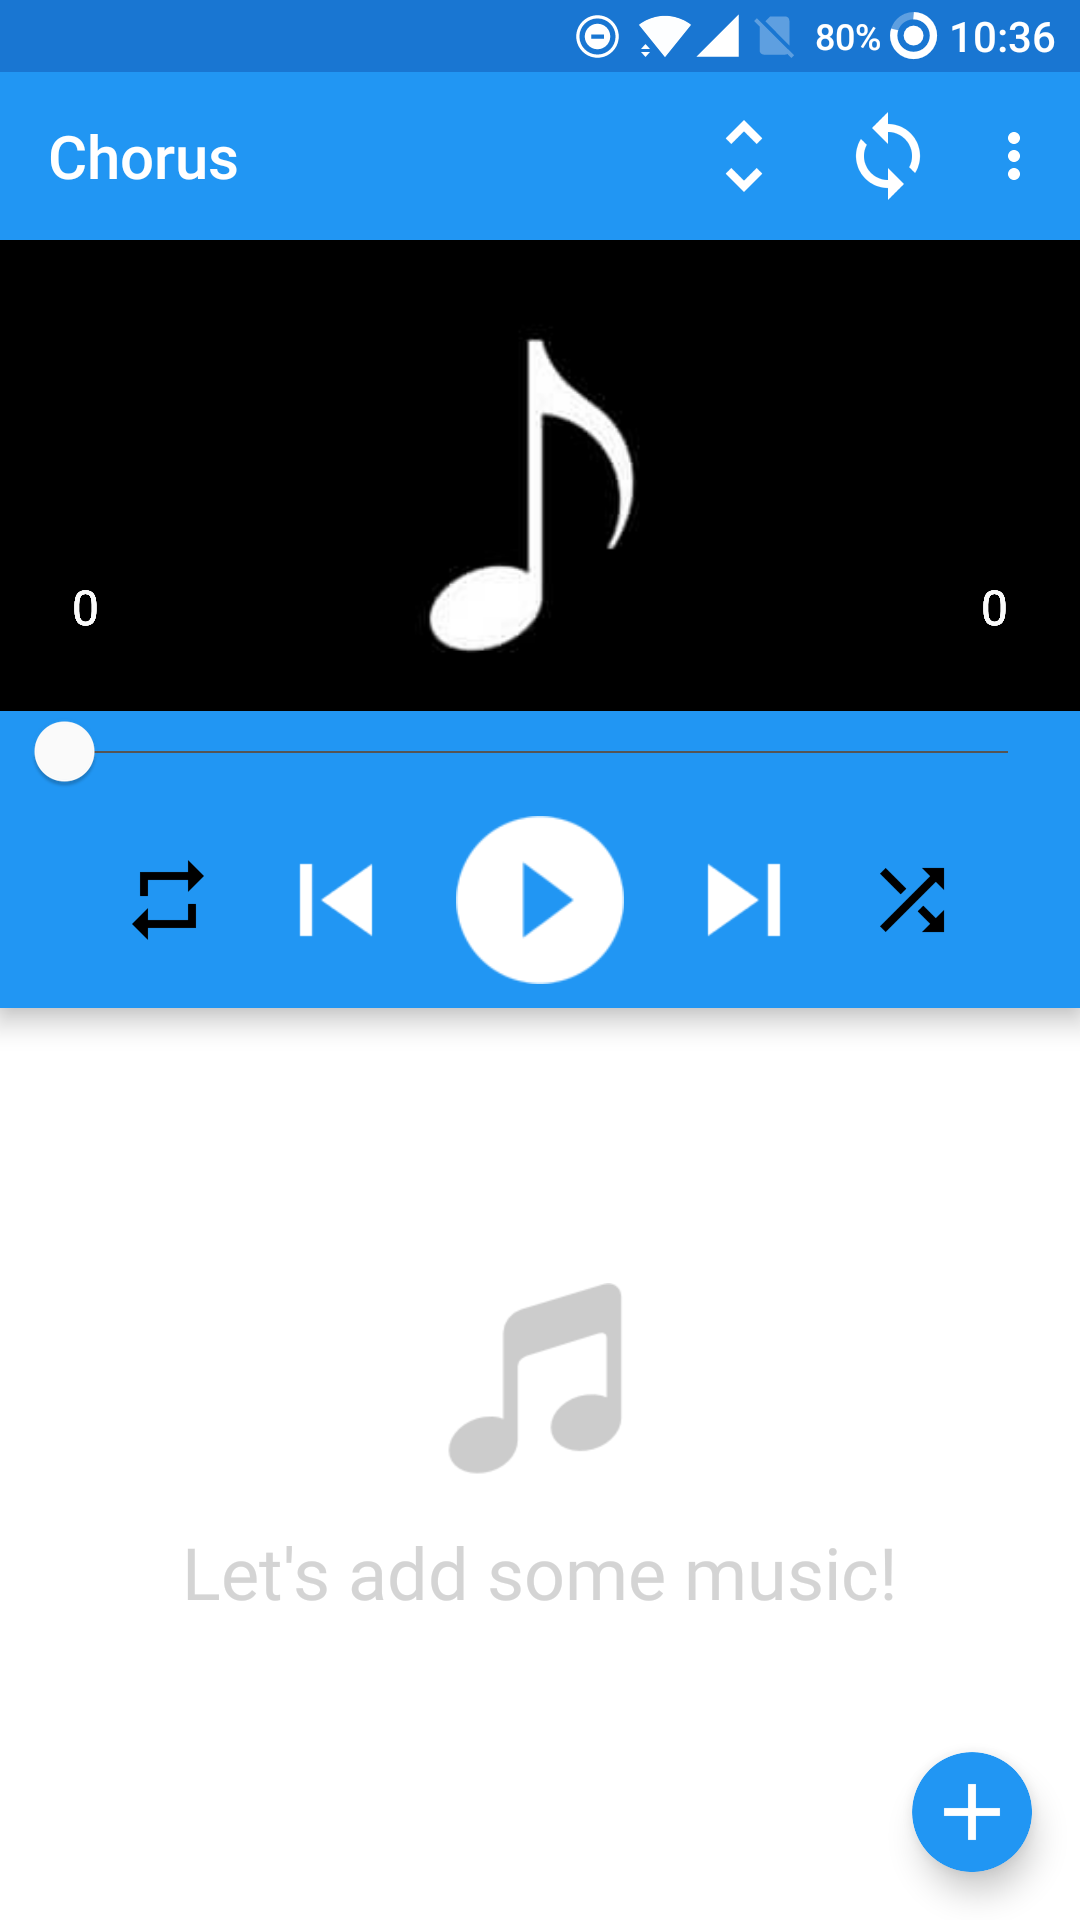
\includegraphics[width=0.65\textwidth]{img/sota/chorus.png}}
        \caption{A screenshot of Chorus when the app is opened.}\label{fig:chorus_screenshot}
    \end{minipage}
    \hfill
    \begin{minipage}[b]{0.45\textwidth}
        \centering
        \fbox{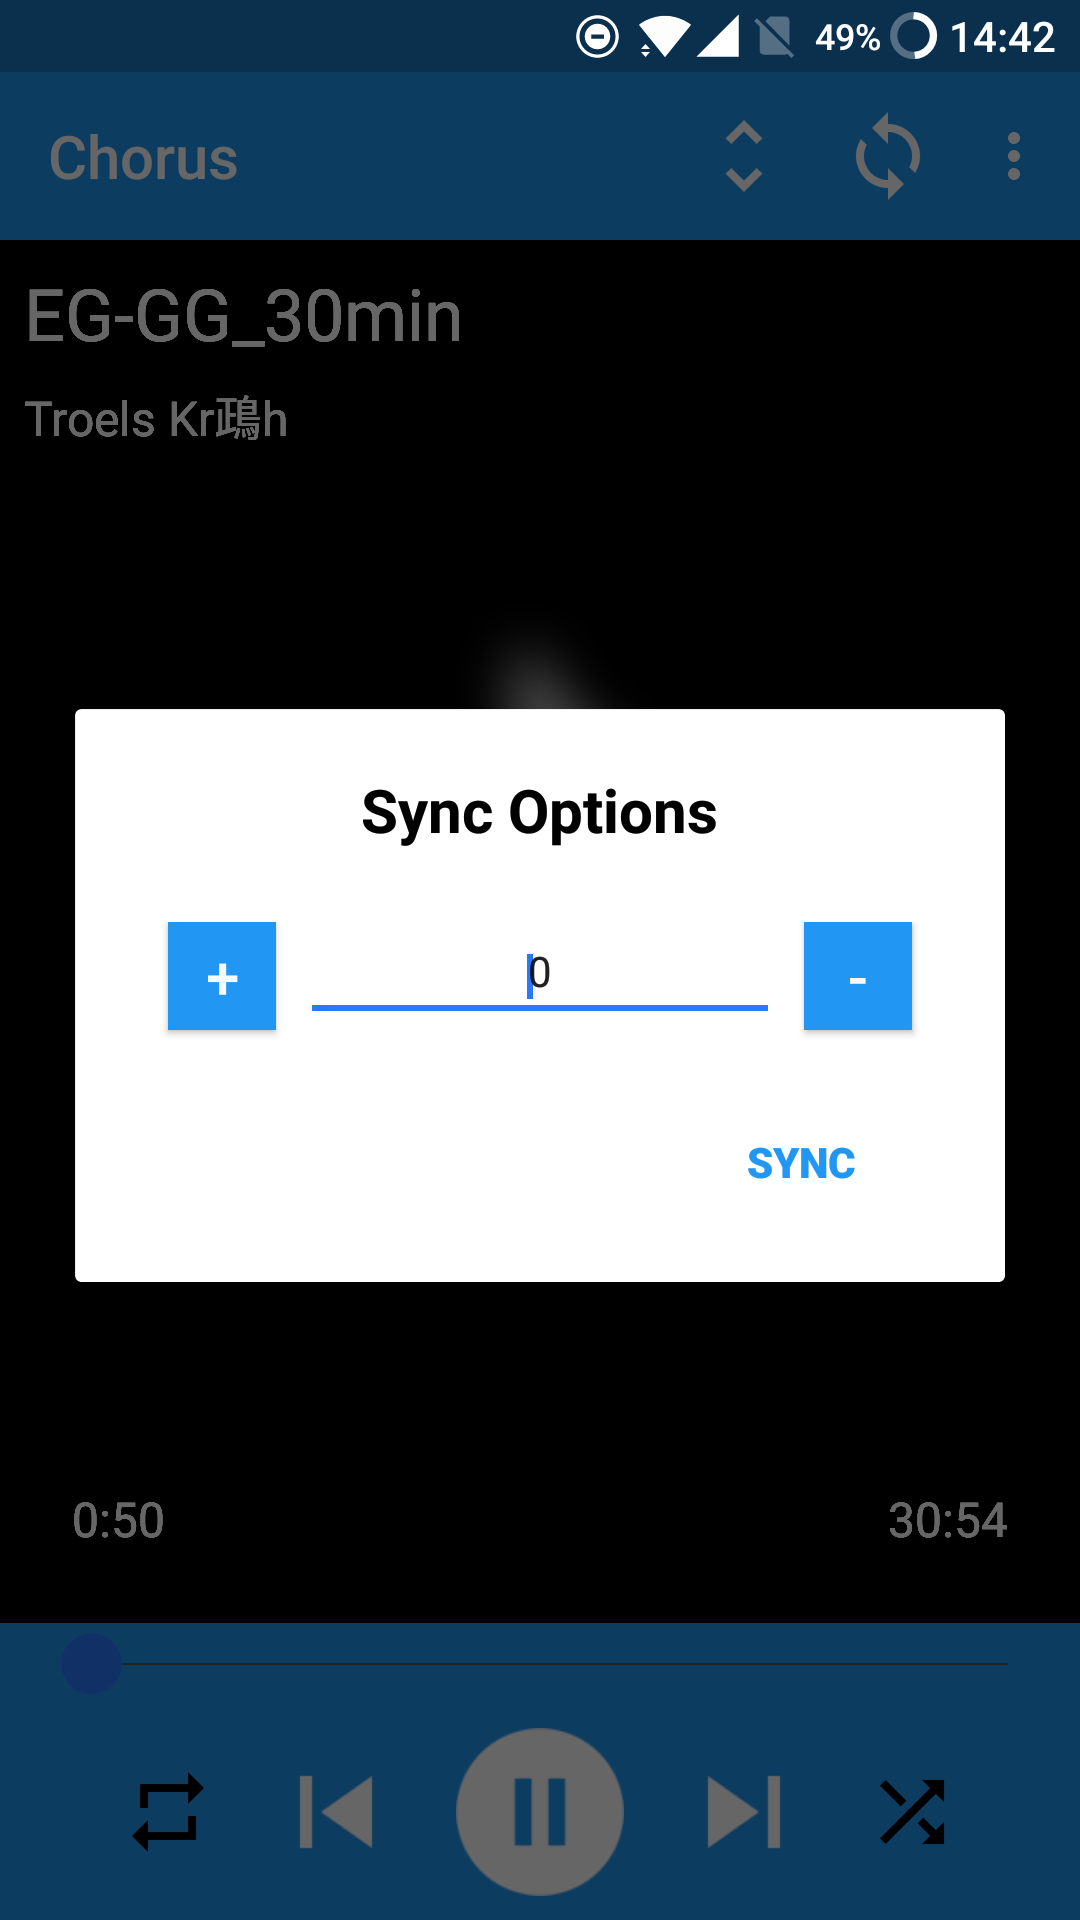
\includegraphics[width=0.65\textwidth]{img/sota/chorus_slider.png}}
        \caption{A screenshot of Chorus' synchronization slider.}\label{fig:chorus_slider}
    \end{minipage}
\end{figure}

\subsection{App Comparison}\label{ssec:app_comparison}
To determine what makes these apps state of the art,
we look at their vital features.
These vital features are the user rating, last update date, supported devices, media source, and connectivity.
We look at these features since we find them important to mobile apps and are factors where the apps can be separated and evaluated.
There do also exist other features of the apps, but we deem these are the most important ones. 
In \cref{tab:sota_comp}, a comparison of the apps can be seen. 

To start with Chorus, it does not support other devices than Android, narrowing down the supported devices compared to SoundSeeder and AmpMe.
Furthermore it only supports local media as music source, requiring all media to be played to be on the device. 
Chorus also has a lower rating than SoundSeeder and AmpMe, which indicates dissatisfied users,
and the last update happened on 11/5 2015 indicating that it is abandoned. 
On the other hand Chorus streams via WiFi and Android hotspot, just as SoundSeeder, and it has automatic and manual synchronization.
Since Chorus only supports Android, playback of local media and do not seem to further developed,
we do not deem it as state of the art.

In regard to SoundSeeder and AmpMe, they have their app ratings, Android support, YouTube and local media support in common.
AmpMe supports iOS devices, but SoundSeeder has a Java version which means that it supports all devices running Java, which is an advantage. 
Therefore to be a part of the state of the art, it is important to support different types of devices.

In regard to supported devices, SoundSeeder supports more devices than AmpMe, but AmpMe supports Spotify.
Spotify has around 100 million users, which makes it an important source to support\cite{spotify_subscribers}.
Google Music have not released any official user numbers, but it is expected to be lower than Spotify\cite{googlem_subscribers}.
On the other hand SoundSeeder supports external sources, so a source supporting Spotify could be used with SoundSeeder that way.
This means that it is important to support popular and widely used music sources to be considered state of the art.

SoundSeeder supports streaming via WiFi or Android hotspot. 
This means that all devices have to be on the same network and have connection to each other,
which can be an issue in larger network configurations, where clients can be restricted from communicating with each other,
which is the case at Aalborg University.
AmpMe does not have this restriction since it uses an Internet connection, this does have the restriction of using mobile data.
Furthermore if slow mobile data is used it can cause problems with the synchronization, but so can Internet via WiFi. 
As both solutions have their respective restrictions we deem that both using WiFi/hotspot and Internet is a part of the state of the art.

Both SoundSeeder and AmpMe synchronizes automatically upon created connection.
In the case that the synchronization becomes skewed, both apps have the possibility of manually synchronize and to set a synchronization offset.
Since there is a need for manual synchronization options, this could mean that the automatic synchronization can at times be faulty,
but it is a good alternative to either disconnect and reconnect or wait for the automatic synchronization synchronize by itself.
Therefore to be a part of the state of the art, an app have to be able to both automatically and manually synchronize.
The actual performance of the synchronization, in SoundSeeder and AmpMe will be tested in a later section.


\begin{table}
    \scalebox{0.9}{
    \begin{tabular}{l|l|l|p{2.2cm}|p{2.5cm}|p{2.4cm}|p{2.0cm}|}
                    & \multirow{2}{*}{Rating}    & \multirow{2}{*}{Last update}   & Supported devices & \multirow{2}{*}{Media source} & \multirow{2}{*}{Connectivity} & \multirow{2}{*}{Pricing}  \\
        \toprule

        \multirow{7}{*}{SoundSeeder} & \multirow{7}{*}{3.9 Play Store}    & \multirow{7}{*}{11/11 2016}    & \multirow{6}{*}{Android 4.1$\le$,} & Google Music, & \multirow{6}{*}{WiFi,} &  \multirow{6}{*}{Free (limited),} \\
    & & & \multirow{6}{*}{Java devices} & YouTube, & \multirow{6}{*}{Android hotspot} & \multirow{6}{*}{39.90 DKK} \\
    & & & & external device, & & \\
    & & & & UPnP, & & \\
    & & & & DLNA, & & \\
    & & & & online radio, & & \\
    & & & & local media & & \\ 

    \midrule

        \multirow{4}{*}{AmpMe} & \multirow{3}{*}{4.2 Play Store} & \multirow{3}{*}{30/01 2017} & \multirow{3}{*}{Android 4.1$\le$,} & Spotify, & \multirow{4}{*}{Internet} & \multirow{4}{*}{Free} \\
    & \multirow{3}{*}{4.0 App Store} & \multirow{3}{*}{01/02 2017} & \multirow{3}{*}{iOS 9.0 $\le$} & SoundCloud, & & \\
    & & & & YouTube, & & \\
    & & & & local media & & \\

    \midrule

        \multirow{2}{*}{Chorus} & \multirow{2}{*}{3.3 Play Store} & \multirow{2}{*}{11/5 2015} & \multirow{2}{*}{Android 4.0 $\le$} & \multirow{2}{*}{Local media} & \multirow{1}{*}{WiFi,} & \multirow{2}{*}{Free} \\
    & & & & & \multirow{1}{*}{Android hotspot} & \\

    \bottomrule

    \end{tabular}}
    \caption{Comparison between the apps as of the 13\textsuperscript{th} of February 2017.}\label{tab:sota_comp}
\end{table}

